\chapter{Calculadora Thrift}

\section{Uso de la calculadora}

Para esta práctica usamos un cliente escrito en Ruby que se comunica con un servidor escrito en Python para realizar las siguientes operaciones:

\begin{itemize}
	\item\textbf{Operaciones con escalares:}
		Reciben dos escalares y devuelven otro escalar.
		\begin{itemize}
			\item
				Suma de dos escalares: \texttt{3 + 2}
			\item
				Resta de dos escalares: \texttt{2 - 7}
			\item
				Producto de dos escalares: \texttt{6 * 2}
			\item
				División entera de dos escalares: \texttt{9 / 2}
		\end{itemize}
	\item\textbf{Operaciones con vectores}
		Reciben dos vectores y devuelven otro vector.
		\begin{itemize}
			\item
				Suma de dos vectores: \texttt{(3,5) + (8,7)}
			\item
				Resta de dos vectores: \texttt{(9,1) - (4,2)}
			\item
				Producto de dos vectores: \texttt{(7,3) * (5,5)}
		\end{itemize}
	\item\textbf{Operaciones con matrices}
		Reciben dos matrices y devuelven otra matriz.
		\begin{itemize}
			\item
				Suma de dos matrices: \texttt{[(2,4)(5,6)] + [(6,8)(1,3)]}
			\item
				Resta de dos matrices: \texttt{[(4,4)(8,4)] - [(4,7)(5,2)]}
			\item
				Producto de dos matrices: \texttt{[(7,1)(8,5)] * [(9,4),(2,3)]}
		\end{itemize}
\end{itemize}

Para iniciar el servidor simplemente debemos entrar en su directorio y ejecutarlo con \texttt{python}:

\begin{lstlisting}[language=sh]
python servidor.py
\end{lstlisting}

Todas estas operaciones se introducen como argumentos al cliente.
Debemos tener en cuenta que la \textit{shell} de Linux requiere que escapemos algunos \textit{tokens}.
Por ejemplo:

\begin{lstlisting}[language=sh]
ruby cliente.rb 2 - 7
ruby cliente.rb \(9,1\) - \(4,2\)
ruby cliente.rb \[\(7,1\)\(8,5\)\] \* \[\(9,4\),\(2,3\)\]
\end{lstlisting}

\pagebreak

\section{Pruebas de la ejecución}

\begin{figure}[ht!]
\begin{center}
	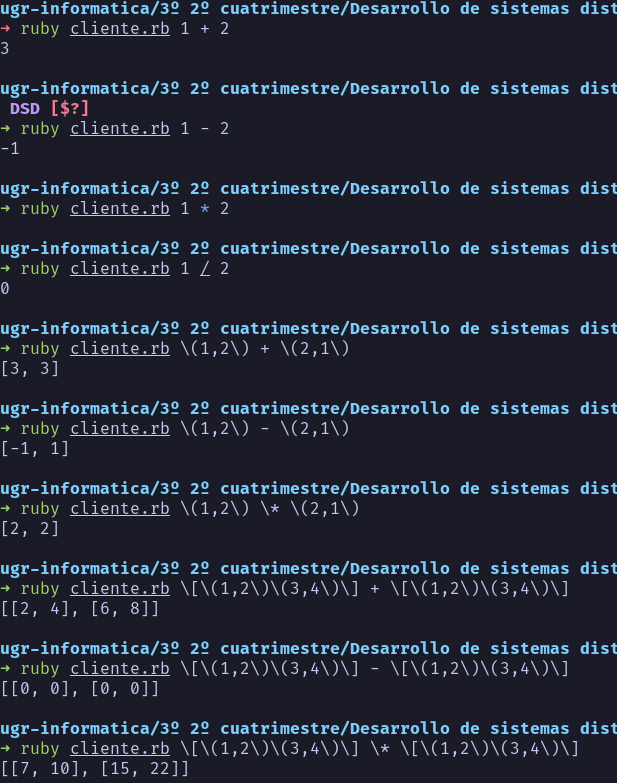
\includegraphics[scale=0.5]{capturas_thrift.png}
\end{center}
\caption{Ejecución de la calculadora con el cliente de Ruby}
\end{figure}
